\paragraph{State Machine Diagrams}
State machine diagrams are used to model the dynamic behavior of individual objects within the system. They illustrate the various states an object can be in, as well as the transitions between those states triggered by events or conditions. In the context of Veritas, state machine diagrams help to define how different components of the system respond to various inputs and how they change their states over time.

The following state machine diagrams represent key components of the Veritas system:

\begin{enumerate}
    \item \textbf{Enterprise Account Creation}
        \begin{itemize}
        \item The Enterprise Account Life Cycle diagram illustrates a hybrid-flow process governing an organization’s journey within the Veritas system. It begins with a vertical approval phase where a Pending Approval registration is reviewed by administrators for activation or rejection. Once in a Fully Functional state, the account enters a horizontal operational phase where data is strictly separated. Administrators can toggle the account into a Suspended state to temporarily restrict access without data loss. Finally, the lifecycle concludes with an account closure process that includes a mandatory 90-day retention period for regulatory compliance and recovery, followed by a permanent purge of all organization records.
        \vspace*{0.5em}
        \begin{figure}[H]
        \centering
        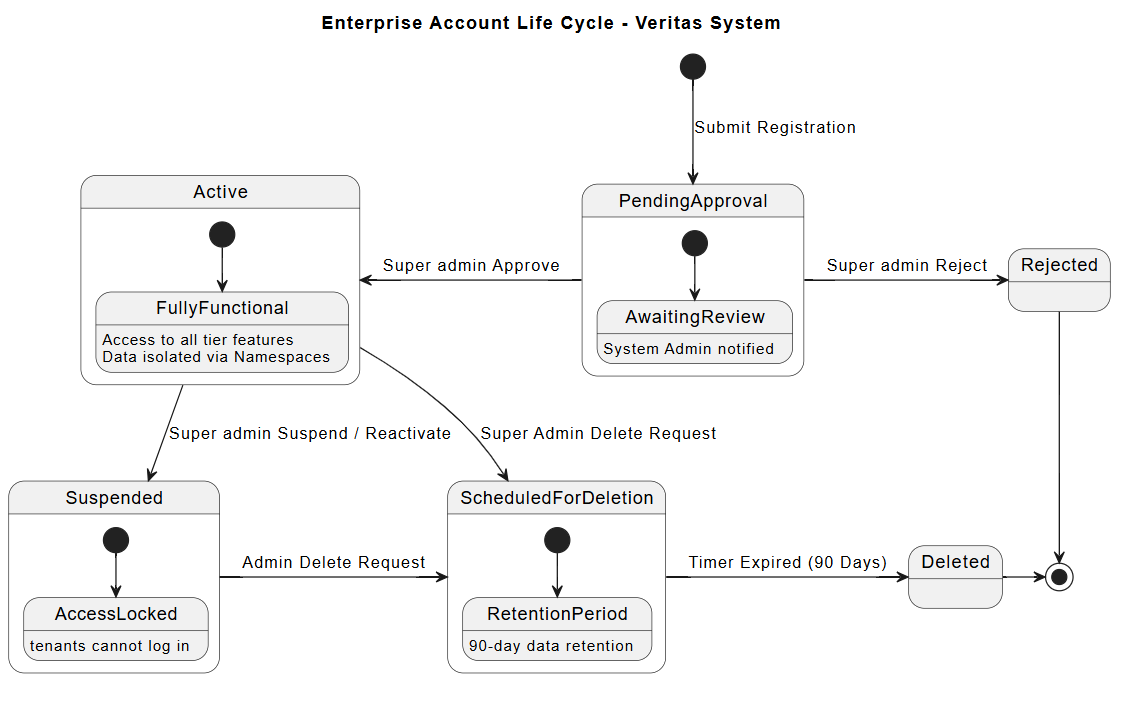
\includegraphics[width=1\linewidth,keepaspectratio]{assets/state_machine_diagrams/Enterprise Account Creation State Machine.png}
        \caption{Enterprise Account Creation State Machine Diagram}
        \label{fig:enterprise-account-creation-state-machine}
        \end{figure}
        \end{itemize}

    \item \textbf{Exam Creation Flow}
        \begin{itemize}
        \item The Exam Status Lifecycle diagram illustrates the progression of an assessment through the Veritas system, transitioning from an initial administrative setup phase to a live operational phase and eventual data preservation. The process begins in the Draft state, where questions and randomization rules are configured, before moving to the Scheduled state once the timing and candidate enrollment are finalized. On the reaching the predefined start time, the system automatically triggers the Active state, enabling real-time monitoring and proctoring for candidates. Upon conclusion, the exam enters the Closed state to facilitate automated AI grading, finally moving to the Archived status where results are preserved as read-only historical records for auditing purposes.
        \vspace*{0.5em}
        \begin{figure}[H]
        \centering
        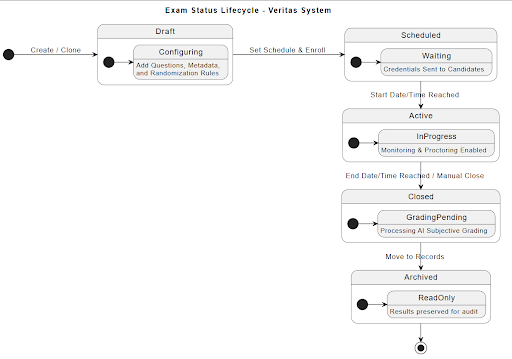
\includegraphics[width=1\linewidth,keepaspectratio]{assets/state_machine_diagrams/Exam Creation State Machine.png}
        \caption{Exam Creation State Machine Diagram}
        \label{fig:exam-creation-state-machine}
        \end{figure}
        \end{itemize}

    \item \textbf{Candidate Examination Flow}
        \begin{itemize}
        \item The Candidate Examination Flow diagram illustrates the student’s journey through a secure assessment session . The process moves from Awaiting Start to an Active Exam state, where the system manages question navigation and background data syncing. To ensure stability on unreliable networks, a Connection Lost state allows for local answer queuing and automatic background synchronization once the connection is restored. The session can be abruptly ended via a Forced Terminated state if a major integrity violation is detected; otherwise, it proceeds to a Reviewing phase before finalization. The lifecycle concludes at the Submitted state, marking the successful and secure completion of the exam.
        \vspace*{0.5em}
        \begin{figure}[H]
        \centering
        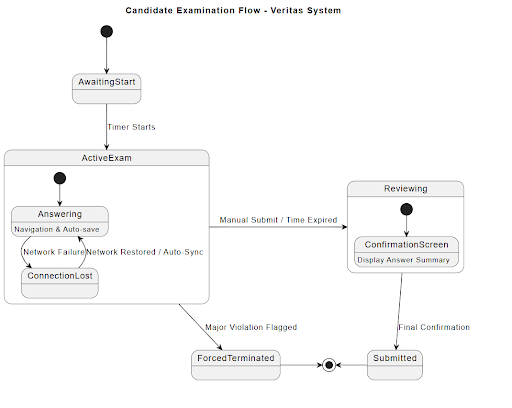
\includegraphics[width=1\linewidth,keepaspectratio]{assets/state_machine_diagrams/Candidate Examination State Machine.png}
        \caption{Candidate Examination State Machine Diagram}
        \label{fig:candidate-examination-state-machine}
        \end{figure}
        \end{itemize}
    
    \item \textbf{AI Proctoring Module State Flow}
        \begin{itemize}
        \item The AI Proctoring \& Monitoring diagram illustrates the continuous background surveillance logic used to maintain exam integrity. The process begins in an Active Monitoring state, where the system performs real-time analysis of webcam feeds, mouse movements, and browser activity. When a deviation, such as a tab switch or facial absence, is identified, the system transitions to an Anomaly Detected phase to calculate a risk score and capture evidence. While minor issues allow the system to return to active tracking, persistent or high-severity behaviors move the session into a Flagged state. If the cumulative cheating probability exceeds a set threshold, the system triggers a Critical Violation, alerting administrators and potentially terminating the session to prevent further compromise.
        \vspace*{0.5em}
        \begin{figure}[H]
        \centering
        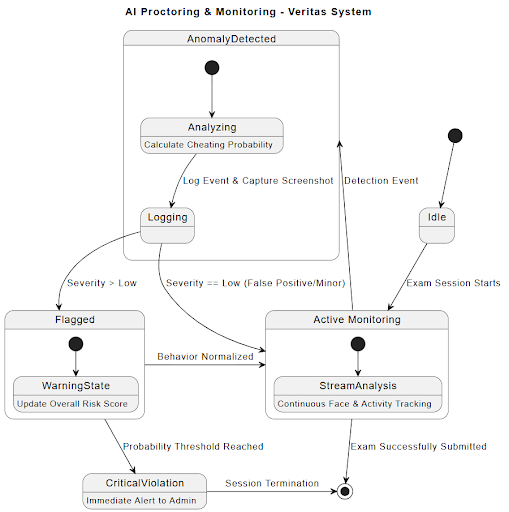
\includegraphics[width=1\linewidth,keepaspectratio]{assets/state_machine_diagrams/AI Proctoring State Machine.png}
        \caption{AI Proctoring and Monitoring State Machine Diagram}
        \label{fig:ai-proctoring-state-machine}
        \end{figure}
        \end{itemize}
    
    \item \textbf{Grading Module Flow}
        \begin{itemize}
        \item The Grading \& Results Lifecycle diagram illustrates the progression from exam submission to performance reporting. Upon submission, the Pending Grading state uses AI to evaluate responses, with a guarded path for authorized manual override when AI confidence is low. The process then moves to Analytics Calculation, where the system generates rankings and performs variance analysis to compare outcomes against baseline metrics. The lifecycle concludes in the Reporting phase with the delivery of personalized feedback to candidates.
        \vspace*{0.5em}
        \begin{figure}[H]
        \centering
        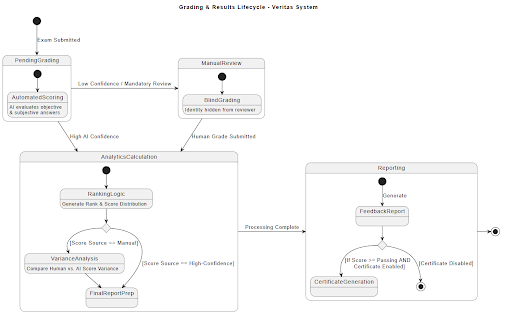
\includegraphics[width=1\linewidth,keepaspectratio]{assets/state_machine_diagrams/Grading and Results State Machine.png}
        \caption{Grading and Results State Machine Diagram}
        \label{fig:grading-results-state-machine}
        \end{figure}
        \end{itemize}
\end{enumerate}